\documentclass[1p]{elsarticle_modified}
%\bibliographystyle{elsarticle-num}

%\usepackage[colorlinks]{hyperref}
%\usepackage{abbrmath_seonhwa} %\Abb, \Ascr, \Acal ,\Abf, \Afrak
\usepackage{amsfonts}
\usepackage{amssymb}
\usepackage{amsmath}
\usepackage{amsthm}
\usepackage{scalefnt}
\usepackage{amsbsy}
\usepackage{kotex}
\usepackage{caption}
\usepackage{subfig}
\usepackage{color}
\usepackage{graphicx}
\usepackage{xcolor} %% white, black, red, green, blue, cyan, magenta, yellow
\usepackage{float}
\usepackage{setspace}
\usepackage{hyperref}

\usepackage{tikz}
\usetikzlibrary{arrows}

\usepackage{multirow}
\usepackage{array} % fixed length table
\usepackage{hhline}

%%%%%%%%%%%%%%%%%%%%%
\makeatletter
\renewcommand*\env@matrix[1][\arraystretch]{%
	\edef\arraystretch{#1}%
	\hskip -\arraycolsep
	\let\@ifnextchar\new@ifnextchar
	\array{*\c@MaxMatrixCols c}}
\makeatother %https://tex.stackexchange.com/questions/14071/how-can-i-increase-the-line-spacing-in-a-matrix
%%%%%%%%%%%%%%%

\usepackage[normalem]{ulem}

\newcommand{\msout}[1]{\ifmmode\text{\sout{\ensuremath{#1}}}\else\sout{#1}\fi}
%SOURCE: \msout is \stkout macro in https://tex.stackexchange.com/questions/20609/strikeout-in-math-mode

\newcommand{\cancel}[1]{
	\ifmmode
	{\color{red}\msout{#1}}
	\else
	{\color{red}\sout{#1}}
	\fi
}

\newcommand{\add}[1]{
	{\color{blue}\uwave{#1}}
}

\newcommand{\replace}[2]{
	\ifmmode
	{\color{red}\msout{#1}}{\color{blue}\uwave{#2}}
	\else
	{\color{red}\sout{#1}}{\color{blue}\uwave{#2}}
	\fi
}

\newcommand{\Sol}{\mathcal{S}} %segment
\newcommand{\D}{D} %diagram
\newcommand{\A}{\mathcal{A}} %arc


%%%%%%%%%%%%%%%%%%%%%%%%%%%%%5 test

\def\sl{\operatorname{\textup{SL}}(2,\Cbb)}
\def\psl{\operatorname{\textup{PSL}}(2,\Cbb)}
\def\quan{\mkern 1mu \triangleright \mkern 1mu}

\theoremstyle{definition}
\newtheorem{thm}{Theorem}[section]
\newtheorem{prop}[thm]{Proposition}
\newtheorem{lem}[thm]{Lemma}
\newtheorem{ques}[thm]{Question}
\newtheorem{cor}[thm]{Corollary}
\newtheorem{defn}[thm]{Definition}
\newtheorem{exam}[thm]{Example}
\newtheorem{rmk}[thm]{Remark}
\newtheorem{alg}[thm]{Algorithm}

\newcommand{\I}{\sqrt{-1}}
\begin{document}

%\begin{frontmatter}
%
%\title{Boundary parabolic representations of knots up to 8 crossings}
%
%%% Group authors per affiliation:
%\author{Yunhi Cho} 
%\address{Department of Mathematics, University of Seoul, Seoul, Korea}
%\ead{yhcho@uos.ac.kr}
%
%
%\author{Seonhwa Kim} %\fnref{s_kim}}
%\address{Center for Geometry and Physics, Institute for Basic Science, Pohang, 37673, Korea}
%\ead{ryeona17@ibs.re.kr}
%
%\author{Hyuk Kim}
%\address{Department of Mathematical Sciences, Seoul National University, Seoul 08826, Korea}
%\ead{hyukkim@snu.ac.kr}
%
%\author{Seokbeom Yoon}
%\address{Department of Mathematical Sciences, Seoul National University, Seoul, 08826,  Korea}
%\ead{sbyoon15@snu.ac.kr}
%
%\begin{abstract}
%We find all boundary parabolic representation of knots up to 8 crossings.
%
%\end{abstract}
%\begin{keyword}
%    \MSC[2010] 57M25 
%\end{keyword}
%
%\end{frontmatter}

%\linenumbers
%\tableofcontents
%
\newcommand\colored[1]{\textcolor{white}{\rule[-0.35ex]{0.8em}{1.4ex}}\kern-0.8em\color{red} #1}%
%\newcommand\colored[1]{\textcolor{white}{ #1}\kern-2.17ex	\textcolor{white}{ #1}\kern-1.81ex	\textcolor{white}{ #1}\kern-2.15ex\color{red}#1	}

{\Large $\underline{12a_{0635}~(K12a_{0635})}$}

\setlength{\tabcolsep}{10pt}
\renewcommand{\arraystretch}{1.6}
\vspace{1cm}\begin{tabular}{m{100pt}>{\centering\arraybackslash}m{274pt}}
\multirow{5}{120pt}{
	\centering
	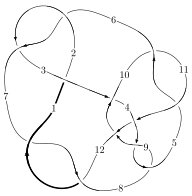
\includegraphics[width=112pt]{../../../GIT/diagram.site/Diagrams/png/1436_12a_0635.png}\\
\ \ \ A knot diagram\footnotemark}&
\allowdisplaybreaks
\textbf{Linearized knot diagam} \\
\cline{2-2}
 &
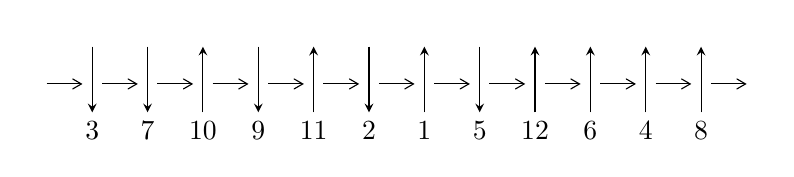
\begin{tikzpicture}[x=20pt, y=17pt]
	% nodes
	\node (C0) at (0, 0) {};
	\node (C1) at (1, 0) {};
	\node (C1U) at (1, +1) {};
	\node (C1D) at (1, -1) {3};

	\node (C2) at (2, 0) {};
	\node (C2U) at (2, +1) {};
	\node (C2D) at (2, -1) {7};

	\node (C3) at (3, 0) {};
	\node (C3U) at (3, +1) {};
	\node (C3D) at (3, -1) {10};

	\node (C4) at (4, 0) {};
	\node (C4U) at (4, +1) {};
	\node (C4D) at (4, -1) {9};

	\node (C5) at (5, 0) {};
	\node (C5U) at (5, +1) {};
	\node (C5D) at (5, -1) {11};

	\node (C6) at (6, 0) {};
	\node (C6U) at (6, +1) {};
	\node (C6D) at (6, -1) {2};

	\node (C7) at (7, 0) {};
	\node (C7U) at (7, +1) {};
	\node (C7D) at (7, -1) {1};

	\node (C8) at (8, 0) {};
	\node (C8U) at (8, +1) {};
	\node (C8D) at (8, -1) {5};

	\node (C9) at (9, 0) {};
	\node (C9U) at (9, +1) {};
	\node (C9D) at (9, -1) {12};

	\node (C10) at (10, 0) {};
	\node (C10U) at (10, +1) {};
	\node (C10D) at (10, -1) {6};

	\node (C11) at (11, 0) {};
	\node (C11U) at (11, +1) {};
	\node (C11D) at (11, -1) {4};

	\node (C12) at (12, 0) {};
	\node (C12U) at (12, +1) {};
	\node (C12D) at (12, -1) {8};
	\node (C13) at (13, 0) {};

	% arrows
	\draw[->,>={angle 60}]
	(C0) edge (C1) (C1) edge (C2) (C2) edge (C3) (C3) edge (C4) (C4) edge (C5) (C5) edge (C6) (C6) edge (C7) (C7) edge (C8) (C8) edge (C9) (C9) edge (C10) (C10) edge (C11) (C11) edge (C12) (C12) edge (C13) ;	\draw[->,>=stealth]
	(C1U) edge (C1D) (C2U) edge (C2D) (C3D) edge (C3U) (C4U) edge (C4D) (C5D) edge (C5U) (C6U) edge (C6D) (C7D) edge (C7U) (C8U) edge (C8D) (C9D) edge (C9U) (C10D) edge (C10U) (C11D) edge (C11U) (C12D) edge (C12U) ;
	\end{tikzpicture} \\
\hhline{~~} \\& 
\textbf{Solving Sequence} \\ \cline{2-2} 
 &
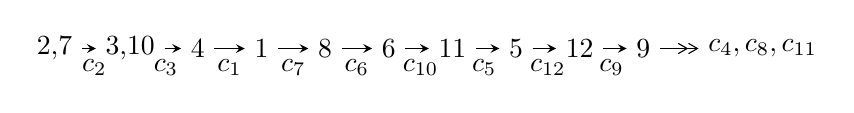
\begin{tikzpicture}[x=23pt, y=7pt]
	% node
	\node (A0) at (-1/8, 0) {2,7};
	\node (A1) at (17/16, 0) {3,10};
	\node (A2) at (17/8, 0) {4};
	\node (A3) at (25/8, 0) {1};
	\node (A4) at (33/8, 0) {8};
	\node (A5) at (41/8, 0) {6};
	\node (A6) at (49/8, 0) {11};
	\node (A7) at (57/8, 0) {5};
	\node (A8) at (65/8, 0) {12};
	\node (A9) at (73/8, 0) {9};
	\node (C1) at (1/2, -1) {$c_{2}$};
	\node (C2) at (13/8, -1) {$c_{3}$};
	\node (C3) at (21/8, -1) {$c_{1}$};
	\node (C4) at (29/8, -1) {$c_{7}$};
	\node (C5) at (37/8, -1) {$c_{6}$};
	\node (C6) at (45/8, -1) {$c_{10}$};
	\node (C7) at (53/8, -1) {$c_{5}$};
	\node (C8) at (61/8, -1) {$c_{12}$};
	\node (C9) at (69/8, -1) {$c_{9}$};
	\node (A10) at (11, 0) {$c_{4},c_{8},c_{11}$};

	% edge
	\draw[->,>=stealth]	
	(A0) edge (A1) (A1) edge (A2) (A2) edge (A3) (A3) edge (A4) (A4) edge (A5) (A5) edge (A6) (A6) edge (A7) (A7) edge (A8) (A8) edge (A9) ;
	\draw[->>,>={angle 60}]	
	(A9) edge (A10);
\end{tikzpicture} \\ 

\end{tabular} \\

\footnotetext{
The image of knot diagram is generated by the software ``\textbf{Draw programme}" developed by Andrew Bartholomew(\url{http://www.layer8.co.uk/maths/draw/index.htm\#Running-draw}), where we modified some parts for our purpose(\url{https://github.com/CATsTAILs/LinksPainter}).
}\phantom \\ \newline 
\centering \textbf{Ideals for irreducible components\footnotemark of $X_{\text{par}}$} 
 
\begin{align*}
I^u_{1}&=\langle 
-3.40397\times10^{99} u^{123}+5.19308\times10^{98} u^{122}+\cdots+3.43279\times10^{98} b+2.80609\times10^{100},\\
\phantom{I^u_{1}}&\phantom{= \langle  }-2.32977\times10^{100} u^{123}+3.31992\times10^{99} u^{122}+\cdots+2.40295\times10^{99} a+1.54517\times10^{101},\\
\phantom{I^u_{1}}&\phantom{= \langle  }u^{124}- u^{123}+\cdots-10 u+7\rangle \\
I^u_{2}&=\langle 
-2 u^{23}-3 u^{22}+\cdots+b+3,\;-2 u^{23}-4 u^{22}+\cdots+a+4,\;u^{24}-7 u^{22}+\cdots-3 u^2+1\rangle \\
\\
\end{align*}
\raggedright * 2 irreducible components of $\dim_{\mathbb{C}}=0$, with total 148 representations.\\
\footnotetext{All coefficients of polynomials are rational numbers. But the coefficients are sometimes approximated in decimal forms when there is not enough margin.}
\newpage
\renewcommand{\arraystretch}{1}
\centering \section*{I. $I^u_{1}= \langle -3.40\times10^{99} u^{123}+5.19\times10^{98} u^{122}+\cdots+3.43\times10^{98} b+2.81\times10^{100},\;-2.33\times10^{100} u^{123}+3.32\times10^{99} u^{122}+\cdots+2.40\times10^{99} a+1.55\times10^{101},\;u^{124}- u^{123}+\cdots-10 u+7 \rangle$}
\flushleft \textbf{(i) Arc colorings}\\
\begin{tabular}{m{7pt} m{180pt} m{7pt} m{180pt} }
\flushright $a_{2}=$&$\begin{pmatrix}1\\0\end{pmatrix}$ \\
\flushright $a_{7}=$&$\begin{pmatrix}0\\u\end{pmatrix}$ \\
\flushright $a_{3}=$&$\begin{pmatrix}1\\u^2\end{pmatrix}$ \\
\flushright $a_{10}=$&$\begin{pmatrix}9.69545 u^{123}-1.38160 u^{122}+\cdots+17.6957 u-64.3030\\9.91607 u^{123}-1.51279 u^{122}+\cdots+21.3533 u-81.7439\end{pmatrix}$ \\
\flushright $a_{4}=$&$\begin{pmatrix}-1.32214 u^{123}-1.03175 u^{122}+\cdots-10.3796 u+21.7586\\-4.74984 u^{123}-1.01744 u^{122}+\cdots-28.6100 u+51.0642\end{pmatrix}$ \\
\flushright $a_{1}=$&$\begin{pmatrix}- u^2+1\\- u^4\end{pmatrix}$ \\
\flushright $a_{8}=$&$\begin{pmatrix}u^5-2 u^3+u\\u^7- u^5+u\end{pmatrix}$ \\
\flushright $a_{6}=$&$\begin{pmatrix}u\\u\end{pmatrix}$ \\
\flushright $a_{11}=$&$\begin{pmatrix}7.83332 u^{123}-1.40369 u^{122}+\cdots+17.0457 u-64.9290\\8.05394 u^{123}-1.53487 u^{122}+\cdots+20.7033 u-82.3699\end{pmatrix}$ \\
\flushright $a_{5}=$&$\begin{pmatrix}-6.00946 u^{123}+0.590204 u^{122}+\cdots-16.6985 u+37.3812\\-0.870989 u^{123}+0.301695 u^{122}+\cdots+0.280302 u+4.54417\end{pmatrix}$ \\
\flushright $a_{12}=$&$\begin{pmatrix}- u^8+3 u^6-3 u^4+1\\- u^{10}+2 u^8- u^6-2 u^4+u^2\end{pmatrix}$ \\
\flushright $a_{9}=$&$\begin{pmatrix}7.27947 u^{123}-1.24156 u^{122}+\cdots+12.2294 u-56.5649\\9.78691 u^{123}-1.89303 u^{122}+\cdots+22.0872 u-94.9113\end{pmatrix}$\\&\end{tabular}
\flushleft \textbf{(ii) Obstruction class $= -1$}\\~\\
\flushleft \textbf{(iii) Cusp Shapes $= -25.9880 u^{123}+7.91471 u^{122}+\cdots-61.1217 u+214.607$}\\~\\
\newpage\renewcommand{\arraystretch}{1}
\flushleft \textbf{(iv) u-Polynomials at the component}\newline \\
\begin{tabular}{m{50pt}|m{274pt}}
Crossings & \hspace{64pt}u-Polynomials at each crossing \\
\hline $$\begin{aligned}c_{1}\end{aligned}$$&$\begin{aligned}
&u^{124}+69 u^{123}+\cdots+324 u+49
\end{aligned}$\\
\hline $$\begin{aligned}c_{2},c_{6}\end{aligned}$$&$\begin{aligned}
&u^{124}- u^{123}+\cdots-10 u+7
\end{aligned}$\\
\hline $$\begin{aligned}c_{3}\end{aligned}$$&$\begin{aligned}
&u^{124}+21 u^{122}+\cdots+39652872 u+5579953
\end{aligned}$\\
\hline $$\begin{aligned}c_{4},c_{8}\end{aligned}$$&$\begin{aligned}
&u^{124}+2 u^{123}+\cdots+1136 u+751
\end{aligned}$\\
\hline $$\begin{aligned}c_{5},c_{10}\end{aligned}$$&$\begin{aligned}
&u^{124}+u^{123}+\cdots-3985 u+173
\end{aligned}$\\
\hline $$\begin{aligned}c_{7},c_{12}\end{aligned}$$&$\begin{aligned}
&u^{124}-3 u^{123}+\cdots-14693 u+4312
\end{aligned}$\\
\hline $$\begin{aligned}c_{9}\end{aligned}$$&$\begin{aligned}
&u^{124}+19 u^{123}+\cdots+33 u+1
\end{aligned}$\\
\hline $$\begin{aligned}c_{11}\end{aligned}$$&$\begin{aligned}
&u^{124}-3 u^{123}+\cdots-9 u+2
\end{aligned}$\\
\hline
\end{tabular}\\~\\
\newpage\renewcommand{\arraystretch}{1}
\flushleft \textbf{(v) Riley Polynomials at the component}\newline \\
\begin{tabular}{m{50pt}|m{274pt}}
Crossings & \hspace{64pt}Riley Polynomials at each crossing \\
\hline $$\begin{aligned}c_{1}\end{aligned}$$&$\begin{aligned}
&y^{124}-21 y^{123}+\cdots-81456 y+2401
\end{aligned}$\\
\hline $$\begin{aligned}c_{2},c_{6}\end{aligned}$$&$\begin{aligned}
&y^{124}-69 y^{123}+\cdots-324 y+49
\end{aligned}$\\
\hline $$\begin{aligned}c_{3}\end{aligned}$$&$\begin{aligned}
&y^{124}+42 y^{123}+\cdots+1234397237289356 y+31135875482209
\end{aligned}$\\
\hline $$\begin{aligned}c_{4},c_{8}\end{aligned}$$&$\begin{aligned}
&y^{124}+70 y^{123}+\cdots+4643906 y+564001
\end{aligned}$\\
\hline $$\begin{aligned}c_{5},c_{10}\end{aligned}$$&$\begin{aligned}
&y^{124}+97 y^{123}+\cdots-5851069 y+29929
\end{aligned}$\\
\hline $$\begin{aligned}c_{7},c_{12}\end{aligned}$$&$\begin{aligned}
&y^{124}+111 y^{123}+\cdots-621048393 y+18593344
\end{aligned}$\\
\hline $$\begin{aligned}c_{9}\end{aligned}$$&$\begin{aligned}
&y^{124}-3 y^{123}+\cdots+405 y+1
\end{aligned}$\\
\hline $$\begin{aligned}c_{11}\end{aligned}$$&$\begin{aligned}
&y^{124}- y^{123}+\cdots+71 y+4
\end{aligned}$\\
\hline
\end{tabular}\\~\\
\newpage\flushleft \textbf{(vi) Complex Volumes and Cusp Shapes}
$$\begin{array}{c|c|c}  
\text{Solutions to }I^u_{1}& \I (\text{vol} + \sqrt{-1}CS) & \text{Cusp shape}\\
 \hline 
\begin{aligned}
u &= -0.889763 + 0.507744 I \\
a &= -1.78676 + 1.06679 I \\
b &= -0.76579 + 1.44957 I\end{aligned}
 & \phantom{-}3.58375 + 6.97795 I & \phantom{-0.000000 } 0 \\ \hline\begin{aligned}
u &= -0.889763 - 0.507744 I \\
a &= -1.78676 - 1.06679 I \\
b &= -0.76579 - 1.44957 I\end{aligned}
 & \phantom{-}3.58375 - 6.97795 I & \phantom{-0.000000 } 0 \\ \hline\begin{aligned}
u &= \phantom{-}0.945691 + 0.402211 I \\
a &= -1.29680 - 1.16543 I \\
b &= -0.89408 - 1.38943 I\end{aligned}
 & -0.16775 - 3.71028 I & \phantom{-0.000000 } 0 \\ \hline\begin{aligned}
u &= \phantom{-}0.945691 - 0.402211 I \\
a &= -1.29680 + 1.16543 I \\
b &= -0.89408 + 1.38943 I\end{aligned}
 & -0.16775 + 3.71028 I & \phantom{-0.000000 } 0 \\ \hline\begin{aligned}
u &= -0.876377 + 0.394634 I \\
a &= -1.93332 - 1.22206 I \\
b &= -2.20005 + 0.10005 I\end{aligned}
 & -2.76946 + 2.00721 I & \phantom{-0.000000 } 0 \\ \hline\begin{aligned}
u &= -0.876377 - 0.394634 I \\
a &= -1.93332 + 1.22206 I \\
b &= -2.20005 - 0.10005 I\end{aligned}
 & -2.76946 - 2.00721 I & \phantom{-0.000000 } 0 \\ \hline\begin{aligned}
u &= \phantom{-}1.002310 + 0.295642 I \\
a &= -0.82558 - 1.43356 I \\
b &= -0.89433 - 1.44500 I\end{aligned}
 & \phantom{-}0.02006 - 3.75240 I & \phantom{-0.000000 } 0 \\ \hline\begin{aligned}
u &= \phantom{-}1.002310 - 0.295642 I \\
a &= -0.82558 + 1.43356 I \\
b &= -0.89433 + 1.44500 I\end{aligned}
 & \phantom{-}0.02006 + 3.75240 I & \phantom{-0.000000 } 0 \\ \hline\begin{aligned}
u &= -0.823156 + 0.666752 I \\
a &= -0.746673 - 1.090280 I \\
b &= -1.47353 - 0.15266 I\end{aligned}
 & -1.72676 + 2.56150 I & \phantom{-0.000000 } 0 \\ \hline\begin{aligned}
u &= -0.823156 - 0.666752 I \\
a &= -0.746673 + 1.090280 I \\
b &= -1.47353 + 0.15266 I\end{aligned}
 & -1.72676 - 2.56150 I & \phantom{-0.000000 } 0\\
 \hline 
 \end{array}$$\newpage$$\begin{array}{c|c|c}  
\text{Solutions to }I^u_{1}& \I (\text{vol} + \sqrt{-1}CS) & \text{Cusp shape}\\
 \hline 
\begin{aligned}
u &= -0.853822 + 0.394425 I \\
a &= \phantom{-}1.21120 - 1.31062 I \\
b &= \phantom{-}1.31262 - 2.44704 I\end{aligned}
 & \phantom{-}1.29001 + 5.01865 I & \phantom{-0.000000 } 0 \\ \hline\begin{aligned}
u &= -0.853822 - 0.394425 I \\
a &= \phantom{-}1.21120 + 1.31062 I \\
b &= \phantom{-}1.31262 + 2.44704 I\end{aligned}
 & \phantom{-}1.29001 - 5.01865 I & \phantom{-0.000000 } 0 \\ \hline\begin{aligned}
u &= \phantom{-}0.768921 + 0.534067 I \\
a &= \phantom{-}0.46891 - 1.34274 I \\
b &= \phantom{-}0.921603 - 1.020550 I\end{aligned}
 & \phantom{-}2.71627 - 2.21713 I & \phantom{-0.000000 } 0 \\ \hline\begin{aligned}
u &= \phantom{-}0.768921 - 0.534067 I \\
a &= \phantom{-}0.46891 + 1.34274 I \\
b &= \phantom{-}0.921603 + 1.020550 I\end{aligned}
 & \phantom{-}2.71627 + 2.21713 I & \phantom{-0.000000 } 0 \\ \hline\begin{aligned}
u &= \phantom{-}0.996957 + 0.392353 I \\
a &= -2.20990 - 0.25684 I \\
b &= -1.85601 - 1.40774 I\end{aligned}
 & -1.51548 - 5.69067 I & \phantom{-0.000000 } 0 \\ \hline\begin{aligned}
u &= \phantom{-}0.996957 - 0.392353 I \\
a &= -2.20990 + 0.25684 I \\
b &= -1.85601 + 1.40774 I\end{aligned}
 & -1.51548 + 5.69067 I & \phantom{-0.000000 } 0 \\ \hline\begin{aligned}
u &= \phantom{-}0.764261 + 0.525513 I \\
a &= \phantom{-}1.33835 - 0.92085 I \\
b &= \phantom{-}1.383260 - 0.265113 I\end{aligned}
 & \phantom{-}2.72829 - 2.08959 I & \phantom{-0.000000 } 0 \\ \hline\begin{aligned}
u &= \phantom{-}0.764261 - 0.525513 I \\
a &= \phantom{-}1.33835 + 0.92085 I \\
b &= \phantom{-}1.383260 + 0.265113 I\end{aligned}
 & \phantom{-}2.72829 + 2.08959 I & \phantom{-0.000000 } 0 \\ \hline\begin{aligned}
u &= -1.044810 + 0.245038 I \\
a &= \phantom{-}0.019646 - 0.869080 I \\
b &= -0.552022 + 0.084685 I\end{aligned}
 & -2.52525 + 0.11799 I & \phantom{-0.000000 } 0 \\ \hline\begin{aligned}
u &= -1.044810 - 0.245038 I \\
a &= \phantom{-}0.019646 + 0.869080 I \\
b &= -0.552022 - 0.084685 I\end{aligned}
 & -2.52525 - 0.11799 I & \phantom{-0.000000 } 0\\
 \hline 
 \end{array}$$\newpage$$\begin{array}{c|c|c}  
\text{Solutions to }I^u_{1}& \I (\text{vol} + \sqrt{-1}CS) & \text{Cusp shape}\\
 \hline 
\begin{aligned}
u &= -0.942798 + 0.518681 I \\
a &= \phantom{-}2.26119 + 0.22869 I \\
b &= \phantom{-}2.51625 - 0.87136 I\end{aligned}
 & -3.45548 + 6.95335 I & \phantom{-0.000000 } 0 \\ \hline\begin{aligned}
u &= -0.942798 - 0.518681 I \\
a &= \phantom{-}2.26119 - 0.22869 I \\
b &= \phantom{-}2.51625 + 0.87136 I\end{aligned}
 & -3.45548 - 6.95335 I & \phantom{-0.000000 } 0 \\ \hline\begin{aligned}
u &= \phantom{-}0.550493 + 0.735340 I \\
a &= -0.376700 + 1.173790 I \\
b &= -1.152420 + 0.198373 I\end{aligned}
 & \phantom{-}1.38554 - 5.06519 I & \phantom{-0.000000 } 0 \\ \hline\begin{aligned}
u &= \phantom{-}0.550493 - 0.735340 I \\
a &= -0.376700 - 1.173790 I \\
b &= -1.152420 - 0.198373 I\end{aligned}
 & \phantom{-}1.38554 + 5.06519 I & \phantom{-0.000000 } 0 \\ \hline\begin{aligned}
u &= -0.890883 + 0.191319 I \\
a &= \phantom{-}0.580557 - 0.563384 I \\
b &= \phantom{-}0.052645 - 0.231219 I\end{aligned}
 & -1.53140 + 0.64514 I & \phantom{-0.000000 } 0 \\ \hline\begin{aligned}
u &= -0.890883 - 0.191319 I \\
a &= \phantom{-}0.580557 + 0.563384 I \\
b &= \phantom{-}0.052645 + 0.231219 I\end{aligned}
 & -1.53140 - 0.64514 I & \phantom{-0.000000 } 0 \\ \hline\begin{aligned}
u &= \phantom{-}0.084174 + 0.906109 I \\
a &= -0.931218 - 0.602335 I \\
b &= \phantom{-}0.300318 - 0.615097 I\end{aligned}
 & -5.86891 + 0.84019 I & \phantom{-0.000000 } 0 \\ \hline\begin{aligned}
u &= \phantom{-}0.084174 - 0.906109 I \\
a &= -0.931218 + 0.602335 I \\
b &= \phantom{-}0.300318 + 0.615097 I\end{aligned}
 & -5.86891 - 0.84019 I & \phantom{-0.000000 } 0 \\ \hline\begin{aligned}
u &= \phantom{-}1.089000 + 0.057770 I \\
a &= -0.458899 - 0.176996 I \\
b &= -0.241678 + 1.036480 I\end{aligned}
 & -6.73622 + 1.56313 I & \phantom{-0.000000 } 0 \\ \hline\begin{aligned}
u &= \phantom{-}1.089000 - 0.057770 I \\
a &= -0.458899 + 0.176996 I \\
b &= -0.241678 - 1.036480 I\end{aligned}
 & -6.73622 - 1.56313 I & \phantom{-0.000000 } 0\\
 \hline 
 \end{array}$$\newpage$$\begin{array}{c|c|c}  
\text{Solutions to }I^u_{1}& \I (\text{vol} + \sqrt{-1}CS) & \text{Cusp shape}\\
 \hline 
\begin{aligned}
u &= \phantom{-}0.841789 + 0.308490 I \\
a &= -0.253112 + 1.389370 I \\
b &= -1.010470 - 0.355714 I\end{aligned}
 & -3.35843 - 1.40319 I & \phantom{-0.000000 } 0 \\ \hline\begin{aligned}
u &= \phantom{-}0.841789 - 0.308490 I \\
a &= -0.253112 - 1.389370 I \\
b &= -1.010470 + 0.355714 I\end{aligned}
 & -3.35843 + 1.40319 I & \phantom{-0.000000 } 0 \\ \hline\begin{aligned}
u &= \phantom{-}0.850162 + 0.258786 I \\
a &= \phantom{-}2.34668 + 0.80322 I \\
b &= \phantom{-}2.63478 + 1.53622 I\end{aligned}
 & \phantom{-}0.42242 + 1.57962 I & \phantom{-0.000000 } 0 \\ \hline\begin{aligned}
u &= \phantom{-}0.850162 - 0.258786 I \\
a &= \phantom{-}2.34668 - 0.80322 I \\
b &= \phantom{-}2.63478 - 1.53622 I\end{aligned}
 & \phantom{-}0.42242 - 1.57962 I & \phantom{-0.000000 } 0 \\ \hline\begin{aligned}
u &= -0.165198 + 0.869947 I \\
a &= -1.108970 + 0.817177 I \\
b &= \phantom{-}0.461300 + 0.688223 I\end{aligned}
 & -5.64795 - 4.21433 I & \phantom{-0.000000 } 0 \\ \hline\begin{aligned}
u &= -0.165198 - 0.869947 I \\
a &= -1.108970 - 0.817177 I \\
b &= \phantom{-}0.461300 - 0.688223 I\end{aligned}
 & -5.64795 + 4.21433 I & \phantom{-0.000000 } 0 \\ \hline\begin{aligned}
u &= \phantom{-}0.129719 + 0.875650 I \\
a &= \phantom{-}1.39433 + 0.79952 I \\
b &= -0.315673 + 1.197660 I\end{aligned}
 & -4.74076 + 13.31180 I & \phantom{-0.000000 } 0 \\ \hline\begin{aligned}
u &= \phantom{-}0.129719 - 0.875650 I \\
a &= \phantom{-}1.39433 - 0.79952 I \\
b &= -0.315673 - 1.197660 I\end{aligned}
 & -4.74076 - 13.31180 I & \phantom{-0.000000 } 0 \\ \hline\begin{aligned}
u &= \phantom{-}0.535374 + 0.702510 I \\
a &= -0.70273 - 1.60720 I \\
b &= \phantom{-}0.701838 - 1.188810 I\end{aligned}
 & \phantom{-}1.33621 + 7.70254 I & \phantom{-0.000000 } 0 \\ \hline\begin{aligned}
u &= \phantom{-}0.535374 - 0.702510 I \\
a &= -0.70273 + 1.60720 I \\
b &= \phantom{-}0.701838 + 1.188810 I\end{aligned}
 & \phantom{-}1.33621 - 7.70254 I & \phantom{-0.000000 } 0\\
 \hline 
 \end{array}$$\newpage$$\begin{array}{c|c|c}  
\text{Solutions to }I^u_{1}& \I (\text{vol} + \sqrt{-1}CS) & \text{Cusp shape}\\
 \hline 
\begin{aligned}
u &= \phantom{-}0.963671 + 0.596228 I \\
a &= \phantom{-}1.93246 - 0.19022 I \\
b &= \phantom{-}2.12635 + 1.00542 I\end{aligned}
 & \phantom{-}0.09405 - 12.64730 I & \phantom{-0.000000 } 0 \\ \hline\begin{aligned}
u &= \phantom{-}0.963671 - 0.596228 I \\
a &= \phantom{-}1.93246 + 0.19022 I \\
b &= \phantom{-}2.12635 - 1.00542 I\end{aligned}
 & \phantom{-}0.09405 + 12.64730 I & \phantom{-0.000000 } 0 \\ \hline\begin{aligned}
u &= \phantom{-}0.031930 + 0.850171 I \\
a &= -1.286950 - 0.064024 I \\
b &= \phantom{-}0.384153 - 0.920669 I\end{aligned}
 & -5.65063 + 3.67795 I & \phantom{-0.000000 } 0. - 8.17604 I \\ \hline\begin{aligned}
u &= \phantom{-}0.031930 - 0.850171 I \\
a &= -1.286950 + 0.064024 I \\
b &= \phantom{-}0.384153 + 0.920669 I\end{aligned}
 & -5.65063 - 3.67795 I & \phantom{-0.000000 -}0. + 8.17604 I \\ \hline\begin{aligned}
u &= -0.101551 + 0.843765 I \\
a &= \phantom{-}1.38878 - 0.94054 I \\
b &= -0.214087 - 1.273220 I\end{aligned}
 & -7.69510 - 6.75726 I & \phantom{-0.000000 -}0. + 5.03105 I \\ \hline\begin{aligned}
u &= -0.101551 - 0.843765 I \\
a &= \phantom{-}1.38878 + 0.94054 I \\
b &= -0.214087 + 1.273220 I\end{aligned}
 & -7.69510 + 6.75726 I & \phantom{-0.000000 } 0. - 5.03105 I \\ \hline\begin{aligned}
u &= \phantom{-}0.837971 + 0.022047 I \\
a &= \phantom{-}1.64447 + 1.84336 I \\
b &= \phantom{-}0.67436 + 1.28251 I\end{aligned}
 & \phantom{-}0.40219 + 3.27217 I & -1.49425 - 6.49968 I \\ \hline\begin{aligned}
u &= \phantom{-}0.837971 - 0.022047 I \\
a &= \phantom{-}1.64447 - 1.84336 I \\
b &= \phantom{-}0.67436 - 1.28251 I\end{aligned}
 & \phantom{-}0.40219 - 3.27217 I & -1.49425 + 6.49968 I \\ \hline\begin{aligned}
u &= -1.057650 + 0.510566 I \\
a &= -0.398012 + 0.969133 I \\
b &= -0.25035 + 1.59862 I\end{aligned}
 & \phantom{-}1.56493 + 2.71643 I & \phantom{-0.000000 } 0 \\ \hline\begin{aligned}
u &= -1.057650 - 0.510566 I \\
a &= -0.398012 - 0.969133 I \\
b &= -0.25035 - 1.59862 I\end{aligned}
 & \phantom{-}1.56493 - 2.71643 I & \phantom{-0.000000 } 0\\
 \hline 
 \end{array}$$\newpage$$\begin{array}{c|c|c}  
\text{Solutions to }I^u_{1}& \I (\text{vol} + \sqrt{-1}CS) & \text{Cusp shape}\\
 \hline 
\begin{aligned}
u &= \phantom{-}0.989273 + 0.641767 I \\
a &= -0.793131 + 0.839980 I \\
b &= -1.43009 + 0.17053 I\end{aligned}
 & \phantom{-}0.123254 - 0.138656 I & \phantom{-0.000000 } 0 \\ \hline\begin{aligned}
u &= \phantom{-}0.989273 - 0.641767 I \\
a &= -0.793131 - 0.839980 I \\
b &= -1.43009 - 0.17053 I\end{aligned}
 & \phantom{-}0.123254 + 0.138656 I & \phantom{-0.000000 } 0 \\ \hline\begin{aligned}
u &= -0.094510 + 0.807577 I \\
a &= -0.464865 - 0.390483 I \\
b &= -0.196403 + 1.239820 I\end{aligned}
 & \phantom{-}0.06766 - 6.76111 I & \phantom{-}2.52940 + 6.55266 I \\ \hline\begin{aligned}
u &= -0.094510 - 0.807577 I \\
a &= -0.464865 + 0.390483 I \\
b &= -0.196403 - 1.239820 I\end{aligned}
 & \phantom{-}0.06766 + 6.76111 I & \phantom{-}2.52940 - 6.55266 I \\ \hline\begin{aligned}
u &= -0.730434 + 0.350457 I \\
a &= -2.29314 + 1.56310 I \\
b &= -1.23330 + 0.78842 I\end{aligned}
 & \phantom{-}1.69870 - 1.66163 I & \phantom{-}7.41455 - 1.08859 I \\ \hline\begin{aligned}
u &= -0.730434 - 0.350457 I \\
a &= -2.29314 - 1.56310 I \\
b &= -1.23330 - 0.78842 I\end{aligned}
 & \phantom{-}1.69870 + 1.66163 I & \phantom{-}7.41455 + 1.08859 I \\ \hline\begin{aligned}
u &= -1.194320 + 0.015055 I \\
a &= -0.190612 - 0.231367 I \\
b &= \phantom{-}0.047022 + 0.853370 I\end{aligned}
 & -4.49045 + 6.47677 I & \phantom{-0.000000 } 0 \\ \hline\begin{aligned}
u &= -1.194320 - 0.015055 I \\
a &= -0.190612 + 0.231367 I \\
b &= \phantom{-}0.047022 - 0.853370 I\end{aligned}
 & -4.49045 - 6.47677 I & \phantom{-0.000000 } 0 \\ \hline\begin{aligned}
u &= \phantom{-}0.030886 + 0.803159 I \\
a &= -0.381768 + 0.007558 I \\
b &= -0.222971 - 0.985008 I\end{aligned}
 & -3.41325 + 2.13889 I & -0.30087 - 3.11100 I \\ \hline\begin{aligned}
u &= \phantom{-}0.030886 - 0.803159 I \\
a &= -0.381768 - 0.007558 I \\
b &= -0.222971 + 0.985008 I\end{aligned}
 & -3.41325 - 2.13889 I & -0.30087 + 3.11100 I\\
 \hline 
 \end{array}$$\newpage$$\begin{array}{c|c|c}  
\text{Solutions to }I^u_{1}& \I (\text{vol} + \sqrt{-1}CS) & \text{Cusp shape}\\
 \hline 
\begin{aligned}
u &= -0.603352 + 0.525352 I \\
a &= \phantom{-}1.34188 - 0.48358 I \\
b &= \phantom{-}0.68124 - 1.48669 I\end{aligned}
 & \phantom{-}4.39388 - 2.75837 I & \phantom{-}8.32431 + 1.65329 I \\ \hline\begin{aligned}
u &= -0.603352 - 0.525352 I \\
a &= \phantom{-}1.34188 + 0.48358 I \\
b &= \phantom{-}0.68124 + 1.48669 I\end{aligned}
 & \phantom{-}4.39388 + 2.75837 I & \phantom{-}8.32431 - 1.65329 I \\ \hline\begin{aligned}
u &= -1.152550 + 0.380660 I \\
a &= -0.029035 - 0.952780 I \\
b &= -0.172822 - 0.501079 I\end{aligned}
 & -3.38514 + 0.72503 I & \phantom{-0.000000 } 0 \\ \hline\begin{aligned}
u &= -1.152550 - 0.380660 I \\
a &= -0.029035 + 0.952780 I \\
b &= -0.172822 + 0.501079 I\end{aligned}
 & -3.38514 - 0.72503 I & \phantom{-0.000000 } 0 \\ \hline\begin{aligned}
u &= -0.015556 + 0.785715 I \\
a &= -1.66867 + 0.26406 I \\
b &= \phantom{-}0.448769 + 0.777216 I\end{aligned}
 & -5.42277 - 0.55359 I & -0.973571 - 0.814051 I \\ \hline\begin{aligned}
u &= -0.015556 - 0.785715 I \\
a &= -1.66867 - 0.26406 I \\
b &= \phantom{-}0.448769 - 0.777216 I\end{aligned}
 & -5.42277 + 0.55359 I & -0.973571 + 0.814051 I \\ \hline\begin{aligned}
u &= -0.032020 + 0.781364 I \\
a &= \phantom{-}2.14449 + 0.28280 I \\
b &= \phantom{-}0.732638 + 0.220976 I\end{aligned}
 & -1.35725 - 3.79869 I & \phantom{-}1.65172 + 4.10455 I \\ \hline\begin{aligned}
u &= -0.032020 - 0.781364 I \\
a &= \phantom{-}2.14449 - 0.28280 I \\
b &= \phantom{-}0.732638 - 0.220976 I\end{aligned}
 & -1.35725 + 3.79869 I & \phantom{-}1.65172 - 4.10455 I \\ \hline\begin{aligned}
u &= \phantom{-}0.170088 + 0.730003 I \\
a &= -0.071230 + 0.676753 I \\
b &= -0.731808 + 0.468895 I\end{aligned}
 & \phantom{-}0.37028 + 2.87213 I & \phantom{-}1.28510 + 0.62817 I \\ \hline\begin{aligned}
u &= \phantom{-}0.170088 - 0.730003 I \\
a &= -0.071230 - 0.676753 I \\
b &= -0.731808 - 0.468895 I\end{aligned}
 & \phantom{-}0.37028 - 2.87213 I & \phantom{-}1.28510 - 0.62817 I\\
 \hline 
 \end{array}$$\newpage$$\begin{array}{c|c|c}  
\text{Solutions to }I^u_{1}& \I (\text{vol} + \sqrt{-1}CS) & \text{Cusp shape}\\
 \hline 
\begin{aligned}
u &= -1.172590 + 0.435603 I \\
a &= \phantom{-}0.81891 - 1.24137 I \\
b &= \phantom{-}0.062991 - 0.825371 I\end{aligned}
 & -2.73012 + 1.51532 I & \phantom{-0.000000 } 0 \\ \hline\begin{aligned}
u &= -1.172590 - 0.435603 I \\
a &= \phantom{-}0.81891 + 1.24137 I \\
b &= \phantom{-}0.062991 + 0.825371 I\end{aligned}
 & -2.73012 - 1.51532 I & \phantom{-0.000000 } 0 \\ \hline\begin{aligned}
u &= -0.488087 + 0.554663 I \\
a &= -0.85842 + 2.10605 I \\
b &= \phantom{-}0.504340 + 1.307040 I\end{aligned}
 & -2.20840 - 2.63961 I & \phantom{-}0.25032 + 3.28418 I \\ \hline\begin{aligned}
u &= -0.488087 - 0.554663 I \\
a &= -0.85842 - 2.10605 I \\
b &= \phantom{-}0.504340 - 1.307040 I\end{aligned}
 & -2.20840 + 2.63961 I & \phantom{-}0.25032 - 3.28418 I \\ \hline\begin{aligned}
u &= \phantom{-}1.173020 + 0.480755 I \\
a &= -1.84719 - 0.48053 I \\
b &= -1.54303 - 1.18598 I\end{aligned}
 & -2.39613 - 6.88242 I & \phantom{-0.000000 } 0 \\ \hline\begin{aligned}
u &= \phantom{-}1.173020 - 0.480755 I \\
a &= -1.84719 + 0.48053 I \\
b &= -1.54303 + 1.18598 I\end{aligned}
 & -2.39613 + 6.88242 I & \phantom{-0.000000 } 0 \\ \hline\begin{aligned}
u &= \phantom{-}1.164020 + 0.504706 I \\
a &= -1.117050 + 0.657690 I \\
b &= -1.277680 + 0.300223 I\end{aligned}
 & -2.50842 - 7.51034 I & \phantom{-0.000000 } 0 \\ \hline\begin{aligned}
u &= \phantom{-}1.164020 - 0.504706 I \\
a &= -1.117050 - 0.657690 I \\
b &= -1.277680 - 0.300223 I\end{aligned}
 & -2.50842 + 7.51034 I & \phantom{-0.000000 } 0 \\ \hline\begin{aligned}
u &= -0.562348 + 0.453906 I \\
a &= -0.33839 - 1.87897 I \\
b &= -1.31334 - 0.66272 I\end{aligned}
 & -1.96835 + 1.60122 I & -0.51057 - 4.13265 I \\ \hline\begin{aligned}
u &= -0.562348 - 0.453906 I \\
a &= -0.33839 + 1.87897 I \\
b &= -1.31334 + 0.66272 I\end{aligned}
 & -1.96835 - 1.60122 I & -0.51057 + 4.13265 I\\
 \hline 
 \end{array}$$\newpage$$\begin{array}{c|c|c}  
\text{Solutions to }I^u_{1}& \I (\text{vol} + \sqrt{-1}CS) & \text{Cusp shape}\\
 \hline 
\begin{aligned}
u &= \phantom{-}1.216150 + 0.409530 I \\
a &= -0.809824 - 0.995513 I \\
b &= \phantom{-}0.236122 - 1.216550 I\end{aligned}
 & -3.82762 + 2.56614 I & \phantom{-0.000000 } 0 \\ \hline\begin{aligned}
u &= \phantom{-}1.216150 - 0.409530 I \\
a &= -0.809824 + 0.995513 I \\
b &= \phantom{-}0.236122 + 1.216550 I\end{aligned}
 & -3.82762 - 2.56614 I & \phantom{-0.000000 } 0 \\ \hline\begin{aligned}
u &= \phantom{-}1.206620 + 0.442321 I \\
a &= -0.65156 - 1.85727 I \\
b &= -0.96275 - 2.66504 I\end{aligned}
 & -4.96595 - 0.54583 I & \phantom{-0.000000 } 0 \\ \hline\begin{aligned}
u &= \phantom{-}1.206620 - 0.442321 I \\
a &= -0.65156 + 1.85727 I \\
b &= -0.96275 + 2.66504 I\end{aligned}
 & -4.96595 + 0.54583 I & \phantom{-0.000000 } 0 \\ \hline\begin{aligned}
u &= \phantom{-}1.208230 + 0.450329 I \\
a &= \phantom{-}0.143311 - 0.112206 I \\
b &= \phantom{-}0.931908 + 1.029250 I\end{aligned}
 & -8.99309 - 3.85792 I & \phantom{-0.000000 } 0 \\ \hline\begin{aligned}
u &= \phantom{-}1.208230 - 0.450329 I \\
a &= \phantom{-}0.143311 + 0.112206 I \\
b &= \phantom{-}0.931908 - 1.029250 I\end{aligned}
 & -8.99309 + 3.85792 I & \phantom{-0.000000 } 0 \\ \hline\begin{aligned}
u &= -1.203870 + 0.469104 I \\
a &= \phantom{-}0.09329 + 1.65147 I \\
b &= -0.15745 + 2.52338 I\end{aligned}
 & -4.77346 + 8.32914 I & \phantom{-0.000000 } 0 \\ \hline\begin{aligned}
u &= -1.203870 - 0.469104 I \\
a &= \phantom{-}0.09329 - 1.65147 I \\
b &= -0.15745 - 2.52338 I\end{aligned}
 & -4.77346 - 8.32914 I & \phantom{-0.000000 } 0 \\ \hline\begin{aligned}
u &= -1.207550 + 0.462777 I \\
a &= \phantom{-}1.74836 - 0.92839 I \\
b &= \phantom{-}1.83396 - 2.26101 I\end{aligned}
 & -8.90383 + 5.05532 I & \phantom{-0.000000 } 0 \\ \hline\begin{aligned}
u &= -1.207550 - 0.462777 I \\
a &= \phantom{-}1.74836 + 0.92839 I \\
b &= \phantom{-}1.83396 + 2.26101 I\end{aligned}
 & -8.90383 - 5.05532 I & \phantom{-0.000000 } 0\\
 \hline 
 \end{array}$$\newpage$$\begin{array}{c|c|c}  
\text{Solutions to }I^u_{1}& \I (\text{vol} + \sqrt{-1}CS) & \text{Cusp shape}\\
 \hline 
\begin{aligned}
u &= -1.215380 + 0.442634 I \\
a &= -0.904898 + 0.542762 I \\
b &= -0.235963 + 0.654580 I\end{aligned}
 & -7.08584 + 2.27065 I & \phantom{-0.000000 } 0 \\ \hline\begin{aligned}
u &= -1.215380 - 0.442634 I \\
a &= -0.904898 - 0.542762 I \\
b &= -0.235963 - 0.654580 I\end{aligned}
 & -7.08584 - 2.27065 I & \phantom{-0.000000 } 0 \\ \hline\begin{aligned}
u &= \phantom{-}1.212780 + 0.469577 I \\
a &= \phantom{-}0.90744 + 1.19643 I \\
b &= \phantom{-}0.30638 + 1.45771 I\end{aligned}
 & -6.89339 - 6.73073 I & \phantom{-0.000000 } 0 \\ \hline\begin{aligned}
u &= \phantom{-}1.212780 - 0.469577 I \\
a &= \phantom{-}0.90744 - 1.19643 I \\
b &= \phantom{-}0.30638 - 1.45771 I\end{aligned}
 & -6.89339 + 6.73073 I & \phantom{-0.000000 } 0 \\ \hline\begin{aligned}
u &= \phantom{-}1.250340 + 0.358838 I \\
a &= -0.154675 + 0.085690 I \\
b &= \phantom{-}0.222334 + 1.125380 I\end{aligned}
 & -10.06870 + 0.09249 I & \phantom{-0.000000 } 0 \\ \hline\begin{aligned}
u &= \phantom{-}1.250340 - 0.358838 I \\
a &= -0.154675 - 0.085690 I \\
b &= \phantom{-}0.222334 - 1.125380 I\end{aligned}
 & -10.06870 - 0.09249 I & \phantom{-0.000000 } 0 \\ \hline\begin{aligned}
u &= \phantom{-}1.239790 + 0.401403 I \\
a &= \phantom{-}0.837353 + 0.127179 I \\
b &= \phantom{-}0.201578 - 0.766582 I\end{aligned}
 & -11.77270 + 2.46110 I & \phantom{-0.000000 } 0 \\ \hline\begin{aligned}
u &= \phantom{-}1.239790 - 0.401403 I \\
a &= \phantom{-}0.837353 - 0.127179 I \\
b &= \phantom{-}0.201578 + 0.766582 I\end{aligned}
 & -11.77270 - 2.46110 I & \phantom{-0.000000 } 0 \\ \hline\begin{aligned}
u &= -1.205740 + 0.496070 I \\
a &= \phantom{-}0.98021 - 1.36199 I \\
b &= -0.01005 - 1.80166 I\end{aligned}
 & -3.21033 + 11.52210 I & \phantom{-0.000000 } 0 \\ \hline\begin{aligned}
u &= -1.205740 - 0.496070 I \\
a &= \phantom{-}0.98021 + 1.36199 I \\
b &= -0.01005 + 1.80166 I\end{aligned}
 & -3.21033 - 11.52210 I & \phantom{-0.000000 } 0\\
 \hline 
 \end{array}$$\newpage$$\begin{array}{c|c|c}  
\text{Solutions to }I^u_{1}& \I (\text{vol} + \sqrt{-1}CS) & \text{Cusp shape}\\
 \hline 
\begin{aligned}
u &= -0.346470 + 0.598546 I \\
a &= \phantom{-}1.56949 + 0.18723 I \\
b &= \phantom{-}0.643607 - 0.281030 I\end{aligned}
 & \phantom{-}3.57068 + 1.66346 I & \phantom{-}7.95681 - 0.97959 I \\ \hline\begin{aligned}
u &= -0.346470 - 0.598546 I \\
a &= \phantom{-}1.56949 - 0.18723 I \\
b &= \phantom{-}0.643607 + 0.281030 I\end{aligned}
 & \phantom{-}3.57068 - 1.66346 I & \phantom{-}7.95681 + 0.97959 I \\ \hline\begin{aligned}
u &= -1.261730 + 0.381247 I \\
a &= \phantom{-}0.550601 - 0.130699 I \\
b &= -0.158238 + 0.822053 I\end{aligned}
 & -9.06425 - 9.00214 I & \phantom{-0.000000 } 0 \\ \hline\begin{aligned}
u &= -1.261730 - 0.381247 I \\
a &= \phantom{-}0.550601 + 0.130699 I \\
b &= -0.158238 - 0.822053 I\end{aligned}
 & -9.06425 + 9.00214 I & \phantom{-0.000000 } 0 \\ \hline\begin{aligned}
u &= -1.217400 + 0.506078 I \\
a &= -2.07512 + 1.15288 I \\
b &= -2.12363 + 2.21754 I\end{aligned}
 & -11.0212 + 11.6591 I & \phantom{-0.000000 } 0 \\ \hline\begin{aligned}
u &= -1.217400 - 0.506078 I \\
a &= -2.07512 - 1.15288 I \\
b &= -2.12363 - 2.21754 I\end{aligned}
 & -11.0212 - 11.6591 I & \phantom{-0.000000 } 0 \\ \hline\begin{aligned}
u &= -1.241340 + 0.444472 I \\
a &= -0.016637 + 0.324766 I \\
b &= \phantom{-}0.887868 - 0.518383 I\end{aligned}
 & -9.48502 + 0.89689 I & \phantom{-0.000000 } 0 \\ \hline\begin{aligned}
u &= -1.241340 - 0.444472 I \\
a &= -0.016637 - 0.324766 I \\
b &= \phantom{-}0.887868 + 0.518383 I\end{aligned}
 & -9.48502 - 0.89689 I & \phantom{-0.000000 } 0 \\ \hline\begin{aligned}
u &= \phantom{-}0.097616 + 0.674455 I \\
a &= \phantom{-}0.713694 + 0.416425 I \\
b &= -0.503777 + 1.132830 I\end{aligned}
 & \phantom{-}0.65401 + 2.46549 I & \phantom{-}5.02445 - 1.80014 I \\ \hline\begin{aligned}
u &= \phantom{-}0.097616 - 0.674455 I \\
a &= \phantom{-}0.713694 - 0.416425 I \\
b &= -0.503777 - 1.132830 I\end{aligned}
 & \phantom{-}0.65401 - 2.46549 I & \phantom{-}5.02445 + 1.80014 I\\
 \hline 
 \end{array}$$\newpage$$\begin{array}{c|c|c}  
\text{Solutions to }I^u_{1}& \I (\text{vol} + \sqrt{-1}CS) & \text{Cusp shape}\\
 \hline 
\begin{aligned}
u &= \phantom{-}1.233200 + 0.477241 I \\
a &= \phantom{-}1.51555 + 1.07618 I \\
b &= \phantom{-}1.31004 + 2.29998 I\end{aligned}
 & -9.24636 - 8.43893 I & \phantom{-0.000000 } 0 \\ \hline\begin{aligned}
u &= \phantom{-}1.233200 - 0.477241 I \\
a &= \phantom{-}1.51555 - 1.07618 I \\
b &= \phantom{-}1.31004 - 2.29998 I\end{aligned}
 & -9.24636 + 8.43893 I & \phantom{-0.000000 } 0 \\ \hline\begin{aligned}
u &= -1.215910 + 0.536328 I \\
a &= \phantom{-}1.46121 - 0.53131 I \\
b &= \phantom{-}1.75921 - 1.56137 I\end{aligned}
 & -8.80606 + 9.34534 I & \phantom{-0.000000 } 0 \\ \hline\begin{aligned}
u &= -1.215910 - 0.536328 I \\
a &= \phantom{-}1.46121 + 0.53131 I \\
b &= \phantom{-}1.75921 + 1.56137 I\end{aligned}
 & -8.80606 - 9.34534 I & \phantom{-0.000000 } 0 \\ \hline\begin{aligned}
u &= \phantom{-}1.224110 + 0.524751 I \\
a &= -1.92450 - 1.07444 I \\
b &= -1.94585 - 2.26335 I\end{aligned}
 & -8.0296 - 18.3915 I & \phantom{-0.000000 } 0 \\ \hline\begin{aligned}
u &= \phantom{-}1.224110 - 0.524751 I \\
a &= -1.92450 + 1.07444 I \\
b &= -1.94585 + 2.26335 I\end{aligned}
 & -8.0296 + 18.3915 I & \phantom{-0.000000 } 0 \\ \hline\begin{aligned}
u &= -1.277340 + 0.411628 I \\
a &= -0.258038 - 0.020094 I \\
b &= \phantom{-}0.084685 - 0.846740 I\end{aligned}
 & -10.11280 + 3.75612 I & \phantom{-0.000000 } 0 \\ \hline\begin{aligned}
u &= -1.277340 - 0.411628 I \\
a &= -0.258038 + 0.020094 I \\
b &= \phantom{-}0.084685 + 0.846740 I\end{aligned}
 & -10.11280 - 3.75612 I & \phantom{-0.000000 } 0 \\ \hline\begin{aligned}
u &= \phantom{-}1.248000 + 0.508745 I \\
a &= \phantom{-}1.25587 + 0.67417 I \\
b &= \phantom{-}1.43654 + 1.48601 I\end{aligned}
 & -9.40797 - 5.92605 I & \phantom{-0.000000 } 0 \\ \hline\begin{aligned}
u &= \phantom{-}1.248000 - 0.508745 I \\
a &= \phantom{-}1.25587 - 0.67417 I \\
b &= \phantom{-}1.43654 - 1.48601 I\end{aligned}
 & -9.40797 + 5.92605 I & \phantom{-0.000000 } 0\\
 \hline 
 \end{array}$$\newpage$$\begin{array}{c|c|c}  
\text{Solutions to }I^u_{1}& \I (\text{vol} + \sqrt{-1}CS) & \text{Cusp shape}\\
 \hline 
\begin{aligned}
u &= \phantom{-}0.455083 + 0.372696 I \\
a &= \phantom{-}1.44631 + 0.18307 I \\
b &= \phantom{-}0.768449 + 0.641571 I\end{aligned}
 & \phantom{-}1.164220 + 0.197770 I & \phantom{-}8.79841 - 0.47962 I \\ \hline\begin{aligned}
u &= \phantom{-}0.455083 - 0.372696 I \\
a &= \phantom{-}1.44631 - 0.18307 I \\
b &= \phantom{-}0.768449 - 0.641571 I\end{aligned}
 & \phantom{-}1.164220 - 0.197770 I & \phantom{-}8.79841 + 0.47962 I \\ \hline\begin{aligned}
u &= \phantom{-}0.072835 + 0.491611 I \\
a &= \phantom{-}1.335550 + 0.017512 I \\
b &= -0.529551 + 0.952438 I\end{aligned}
 & \phantom{-}0.66958 + 2.38733 I & \phantom{-}2.94044 - 2.16417 I \\ \hline\begin{aligned}
u &= \phantom{-}0.072835 - 0.491611 I \\
a &= \phantom{-}1.335550 - 0.017512 I \\
b &= -0.529551 - 0.952438 I\end{aligned}
 & \phantom{-}0.66958 - 2.38733 I & \phantom{-}2.94044 + 2.16417 I\\
 \hline 
 \end{array}$$\newpage\newpage\renewcommand{\arraystretch}{1}
\centering \section*{II. $I^u_{2}= \langle -2 u^{23}-3 u^{22}+\cdots+b+3,\;-2 u^{23}-4 u^{22}+\cdots+a+4,\;u^{24}-7 u^{22}+\cdots-3 u^2+1 \rangle$}
\flushleft \textbf{(i) Arc colorings}\\
\begin{tabular}{m{7pt} m{180pt} m{7pt} m{180pt} }
\flushright $a_{2}=$&$\begin{pmatrix}1\\0\end{pmatrix}$ \\
\flushright $a_{7}=$&$\begin{pmatrix}0\\u\end{pmatrix}$ \\
\flushright $a_{3}=$&$\begin{pmatrix}1\\u^2\end{pmatrix}$ \\
\flushright $a_{10}=$&$\begin{pmatrix}2 u^{23}+4 u^{22}+\cdots+12 u^2-4\\2 u^{23}+3 u^{22}+\cdots+8 u^2-3\end{pmatrix}$ \\
\flushright $a_{4}=$&$\begin{pmatrix}-2 u^{23}- u^{22}+\cdots- u+1\\- u^{22}+6 u^{20}+\cdots-2 u^2-2 u\end{pmatrix}$ \\
\flushright $a_{1}=$&$\begin{pmatrix}- u^2+1\\- u^4\end{pmatrix}$ \\
\flushright $a_{8}=$&$\begin{pmatrix}u^5-2 u^3+u\\u^7- u^5+u\end{pmatrix}$ \\
\flushright $a_{6}=$&$\begin{pmatrix}u\\u\end{pmatrix}$ \\
\flushright $a_{11}=$&$\begin{pmatrix}2 u^{23}+3 u^{22}+\cdots+10 u^2-3\\2 u^{23}+2 u^{22}+\cdots+6 u^2-2\end{pmatrix}$ \\
\flushright $a_{5}=$&$\begin{pmatrix}-2 u^{23}-2 u^{22}+\cdots+6 u+4\\u^{23}-2 u^{22}+\cdots+2 u+4\end{pmatrix}$ \\
\flushright $a_{12}=$&$\begin{pmatrix}- u^8+3 u^6-3 u^4+1\\- u^{10}+2 u^8- u^6-2 u^4+u^2\end{pmatrix}$ \\
\flushright $a_{9}=$&$\begin{pmatrix}2 u^{23}+3 u^{22}+\cdots+10 u^2-4\\2 u^{23}+2 u^{22}+\cdots+6 u^2-3\end{pmatrix}$\\&\end{tabular}
\flushleft \textbf{(ii) Obstruction class $= 1$}\\~\\
\flushleft \textbf{(iii) Cusp Shapes $= -17 u^{23}- u^{22}+112 u^{21}+6 u^{20}-355 u^{19}-17 u^{18}+649 u^{17}+26 u^{16}-700 u^{15}-19 u^{14}+333 u^{13}-3 u^{12}+164 u^{11}+33 u^{10}-370 u^9-68 u^8+212 u^7+81 u^6+2 u^5-43 u^4-60 u^3-3 u^2+26 u+5$}\\~\\
\newpage\renewcommand{\arraystretch}{1}
\flushleft \textbf{(iv) u-Polynomials at the component}\newline \\
\begin{tabular}{m{50pt}|m{274pt}}
Crossings & \hspace{64pt}u-Polynomials at each crossing \\
\hline $$\begin{aligned}c_{1}\end{aligned}$$&$\begin{aligned}
&u^{24}-14 u^{23}+\cdots-6 u+1
\end{aligned}$\\
\hline $$\begin{aligned}c_{2}\end{aligned}$$&$\begin{aligned}
&u^{24}-7 u^{22}+\cdots-3 u^2+1
\end{aligned}$\\
\hline $$\begin{aligned}c_{3}\end{aligned}$$&$\begin{aligned}
&u^{24}+u^{23}+\cdots+2 u+1
\end{aligned}$\\
\hline $$\begin{aligned}c_{4}\end{aligned}$$&$\begin{aligned}
&u^{24}+u^{23}+\cdots+12 u^2+1
\end{aligned}$\\
\hline $$\begin{aligned}c_{5}\end{aligned}$$&$\begin{aligned}
&u^{24}+12 u^{22}+\cdots- u+1
\end{aligned}$\\
\hline $$\begin{aligned}c_{6}\end{aligned}$$&$\begin{aligned}
&u^{24}-7 u^{22}+\cdots-3 u^2+1
\end{aligned}$\\
\hline $$\begin{aligned}c_{7}\end{aligned}$$&$\begin{aligned}
&u^{24}+9 u^{22}+\cdots-3 u^2+1
\end{aligned}$\\
\hline $$\begin{aligned}c_{8}\end{aligned}$$&$\begin{aligned}
&u^{24}- u^{23}+\cdots+12 u^2+1
\end{aligned}$\\
\hline $$\begin{aligned}c_{9}\end{aligned}$$&$\begin{aligned}
&u^{24}-2 u^{22}+\cdots+7 u+1
\end{aligned}$\\
\hline $$\begin{aligned}c_{10}\end{aligned}$$&$\begin{aligned}
&u^{24}+12 u^{22}+\cdots+u+1
\end{aligned}$\\
\hline $$\begin{aligned}c_{11}\end{aligned}$$&$\begin{aligned}
&u^{24}-2 u^{23}+\cdots- u+1
\end{aligned}$\\
\hline $$\begin{aligned}c_{12}\end{aligned}$$&$\begin{aligned}
&u^{24}+9 u^{22}+\cdots-3 u^2+1
\end{aligned}$\\
\hline
\end{tabular}\\~\\
\newpage\renewcommand{\arraystretch}{1}
\flushleft \textbf{(v) Riley Polynomials at the component}\newline \\
\begin{tabular}{m{50pt}|m{274pt}}
Crossings & \hspace{64pt}Riley Polynomials at each crossing \\
\hline $$\begin{aligned}c_{1}\end{aligned}$$&$\begin{aligned}
&y^{24}-2 y^{23}+\cdots-10 y+1
\end{aligned}$\\
\hline $$\begin{aligned}c_{2},c_{6}\end{aligned}$$&$\begin{aligned}
&y^{24}-14 y^{23}+\cdots-6 y+1
\end{aligned}$\\
\hline $$\begin{aligned}c_{3}\end{aligned}$$&$\begin{aligned}
&y^{24}-7 y^{23}+\cdots+2 y+1
\end{aligned}$\\
\hline $$\begin{aligned}c_{4},c_{8}\end{aligned}$$&$\begin{aligned}
&y^{24}+17 y^{23}+\cdots+24 y+1
\end{aligned}$\\
\hline $$\begin{aligned}c_{5},c_{10}\end{aligned}$$&$\begin{aligned}
&y^{24}+24 y^{23}+\cdots+17 y+1
\end{aligned}$\\
\hline $$\begin{aligned}c_{7},c_{12}\end{aligned}$$&$\begin{aligned}
&y^{24}+18 y^{23}+\cdots-6 y+1
\end{aligned}$\\
\hline $$\begin{aligned}c_{9}\end{aligned}$$&$\begin{aligned}
&y^{24}-4 y^{23}+\cdots-9 y+1
\end{aligned}$\\
\hline $$\begin{aligned}c_{11}\end{aligned}$$&$\begin{aligned}
&y^{24}+2 y^{23}+\cdots-7 y+1
\end{aligned}$\\
\hline
\end{tabular}\\~\\
\newpage\flushleft \textbf{(vi) Complex Volumes and Cusp Shapes}
$$\begin{array}{c|c|c}  
\text{Solutions to }I^u_{2}& \I (\text{vol} + \sqrt{-1}CS) & \text{Cusp shape}\\
 \hline 
\begin{aligned}
u &= \phantom{-}0.830087 + 0.607865 I \\
a &= -0.787937 + 1.127550 I \\
b &= -1.48311 + 0.08212 I\end{aligned}
 & -1.31891 - 2.39167 I & \phantom{-}8.22171 + 0.99991 I \\ \hline\begin{aligned}
u &= \phantom{-}0.830087 - 0.607865 I \\
a &= -0.787937 - 1.127550 I \\
b &= -1.48311 - 0.08212 I\end{aligned}
 & -1.31891 + 2.39167 I & \phantom{-}8.22171 - 0.99991 I \\ \hline\begin{aligned}
u &= \phantom{-}0.999057 + 0.347047 I \\
a &= -1.36381 - 1.43525 I \\
b &= -1.19874 - 2.31003 I\end{aligned}
 & -0.26640 - 4.90016 I & -0.41787 + 8.67235 I \\ \hline\begin{aligned}
u &= \phantom{-}0.999057 - 0.347047 I \\
a &= -1.36381 + 1.43525 I \\
b &= -1.19874 + 2.31003 I\end{aligned}
 & -0.26640 + 4.90016 I & -0.41787 - 8.67235 I \\ \hline\begin{aligned}
u &= -0.898344 + 0.216416 I \\
a &= -0.84851 - 1.49922 I \\
b &= -1.331090 + 0.161552 I\end{aligned}
 & -3.88873 + 0.99670 I & -9.19138 + 1.06418 I \\ \hline\begin{aligned}
u &= -0.898344 - 0.216416 I \\
a &= -0.84851 + 1.49922 I \\
b &= -1.331090 - 0.161552 I\end{aligned}
 & -3.88873 - 0.99670 I & -9.19138 - 1.06418 I \\ \hline\begin{aligned}
u &= -0.974569 + 0.527157 I \\
a &= -0.756267 - 0.173046 I \\
b &= -1.314500 + 0.356894 I\end{aligned}
 & \phantom{-}0.995615 + 0.733801 I & \phantom{-}3.68845 - 1.75573 I \\ \hline\begin{aligned}
u &= -0.974569 - 0.527157 I \\
a &= -0.756267 + 0.173046 I \\
b &= -1.314500 - 0.356894 I\end{aligned}
 & \phantom{-}0.995615 - 0.733801 I & \phantom{-}3.68845 + 1.75573 I \\ \hline\begin{aligned}
u &= \phantom{-}0.070130 + 0.855176 I \\
a &= -1.284100 - 0.323500 I \\
b &= \phantom{-}0.379137 - 0.657760 I\end{aligned}
 & -5.48258 + 2.65917 I & \phantom{-}0.432647 - 0.716337 I \\ \hline\begin{aligned}
u &= \phantom{-}0.070130 - 0.855176 I \\
a &= -1.284100 + 0.323500 I \\
b &= \phantom{-}0.379137 + 0.657760 I\end{aligned}
 & -5.48258 - 2.65917 I & \phantom{-}0.432647 + 0.716337 I\\
 \hline 
 \end{array}$$\newpage$$\begin{array}{c|c|c}  
\text{Solutions to }I^u_{2}& \I (\text{vol} + \sqrt{-1}CS) & \text{Cusp shape}\\
 \hline 
\begin{aligned}
u &= -0.612663 + 0.473761 I \\
a &= \phantom{-}0.04247 - 1.73742 I \\
b &= -0.225243 - 0.783401 I\end{aligned}
 & \phantom{-}2.10127 + 3.44984 I & \phantom{-}5.50500 - 5.25186 I \\ \hline\begin{aligned}
u &= -0.612663 - 0.473761 I \\
a &= \phantom{-}0.04247 + 1.73742 I \\
b &= -0.225243 + 0.783401 I\end{aligned}
 & \phantom{-}2.10127 - 3.44984 I & \phantom{-}5.50500 + 5.25186 I \\ \hline\begin{aligned}
u &= \phantom{-}1.161630 + 0.417142 I \\
a &= -0.04559 - 1.76635 I \\
b &= \phantom{-}0.40212 - 1.45647 I\end{aligned}
 & -2.75004 - 0.15086 I & \phantom{-}2.66319 - 3.71566 I \\ \hline\begin{aligned}
u &= \phantom{-}1.161630 - 0.417142 I \\
a &= -0.04559 + 1.76635 I \\
b &= \phantom{-}0.40212 + 1.45647 I\end{aligned}
 & -2.75004 + 0.15086 I & \phantom{-}2.66319 + 3.71566 I \\ \hline\begin{aligned}
u &= -1.160360 + 0.486741 I \\
a &= \phantom{-}1.23692 + 0.81611 I \\
b &= \phantom{-}1.167500 + 0.316108 I\end{aligned}
 & -2.24622 + 8.08592 I & \phantom{-}2.57244 - 12.50899 I \\ \hline\begin{aligned}
u &= -1.160360 - 0.486741 I \\
a &= \phantom{-}1.23692 - 0.81611 I \\
b &= \phantom{-}1.167500 - 0.316108 I\end{aligned}
 & -2.24622 - 8.08592 I & \phantom{-}2.57244 + 12.50899 I \\ \hline\begin{aligned}
u &= \phantom{-}0.707470 + 0.179898 I \\
a &= \phantom{-}2.73022 + 2.10461 I \\
b &= \phantom{-}1.88663 + 1.35622 I\end{aligned}
 & \phantom{-}0.97241 + 2.30300 I & \phantom{-}3.64056 - 4.71970 I \\ \hline\begin{aligned}
u &= \phantom{-}0.707470 - 0.179898 I \\
a &= \phantom{-}2.73022 - 2.10461 I \\
b &= \phantom{-}1.88663 - 1.35622 I\end{aligned}
 & \phantom{-}0.97241 - 2.30300 I & \phantom{-}3.64056 + 4.71970 I \\ \hline\begin{aligned}
u &= -1.241630 + 0.425857 I \\
a &= \phantom{-}0.1166810 + 0.0396087 I \\
b &= \phantom{-}0.777120 - 0.932683 I\end{aligned}
 & -9.45240 + 1.79763 I & -3.66132 - 2.97351 I \\ \hline\begin{aligned}
u &= -1.241630 - 0.425857 I \\
a &= \phantom{-}0.1166810 - 0.0396087 I \\
b &= \phantom{-}0.777120 + 0.932683 I\end{aligned}
 & -9.45240 - 1.79763 I & -3.66132 + 2.97351 I\\
 \hline 
 \end{array}$$\newpage$$\begin{array}{c|c|c}  
\text{Solutions to }I^u_{2}& \I (\text{vol} + \sqrt{-1}CS) & \text{Cusp shape}\\
 \hline 
\begin{aligned}
u &= -0.112951 + 0.674509 I \\
a &= \phantom{-}0.137859 + 0.205443 I \\
b &= \phantom{-}1.066660 + 0.565024 I\end{aligned}
 & \phantom{-}0.69686 - 3.66859 I & \phantom{-}5.64131 + 7.83145 I \\ \hline\begin{aligned}
u &= -0.112951 - 0.674509 I \\
a &= \phantom{-}0.137859 - 0.205443 I \\
b &= \phantom{-}1.066660 - 0.565024 I\end{aligned}
 & \phantom{-}0.69686 + 3.66859 I & \phantom{-}5.64131 - 7.83145 I \\ \hline\begin{aligned}
u &= \phantom{-}1.232150 + 0.493085 I \\
a &= \phantom{-}1.32207 + 0.83590 I \\
b &= \phantom{-}1.37352 + 1.93665 I\end{aligned}
 & -8.96968 - 7.53432 I & -2.09474 + 3.83158 I \\ \hline\begin{aligned}
u &= \phantom{-}1.232150 - 0.493085 I \\
a &= \phantom{-}1.32207 - 0.83590 I \\
b &= \phantom{-}1.37352 - 1.93665 I\end{aligned}
 & -8.96968 + 7.53432 I & -2.09474 - 3.83158 I\\
 \hline 
 \end{array}$$\newpage
\newpage\renewcommand{\arraystretch}{1}
\centering \section*{ III. u-Polynomials}
\begin{tabular}{m{50pt}|m{274pt}}
Crossings & \hspace{64pt}u-Polynomials at each crossing \\
\hline $$\begin{aligned}c_{1}\end{aligned}$$&$\begin{aligned}
&(u^{24}-14 u^{23}+\cdots-6 u+1)(u^{124}+69 u^{123}+\cdots+324 u+49)
\end{aligned}$\\
\hline $$\begin{aligned}c_{2}\end{aligned}$$&$\begin{aligned}
&(u^{24}-7 u^{22}+\cdots-3 u^2+1)(u^{124}- u^{123}+\cdots-10 u+7)
\end{aligned}$\\
\hline $$\begin{aligned}c_{3}\end{aligned}$$&$\begin{aligned}
&(u^{24}+u^{23}+\cdots+2 u+1)\\
&\cdot(u^{124}+21 u^{122}+\cdots+39652872 u+5579953)
\end{aligned}$\\
\hline $$\begin{aligned}c_{4}\end{aligned}$$&$\begin{aligned}
&(u^{24}+u^{23}+\cdots+12 u^2+1)(u^{124}+2 u^{123}+\cdots+1136 u+751)
\end{aligned}$\\
\hline $$\begin{aligned}c_{5}\end{aligned}$$&$\begin{aligned}
&(u^{24}+12 u^{22}+\cdots- u+1)(u^{124}+u^{123}+\cdots-3985 u+173)
\end{aligned}$\\
\hline $$\begin{aligned}c_{6}\end{aligned}$$&$\begin{aligned}
&(u^{24}-7 u^{22}+\cdots-3 u^2+1)(u^{124}- u^{123}+\cdots-10 u+7)
\end{aligned}$\\
\hline $$\begin{aligned}c_{7}\end{aligned}$$&$\begin{aligned}
&(u^{24}+9 u^{22}+\cdots-3 u^2+1)(u^{124}-3 u^{123}+\cdots-14693 u+4312)
\end{aligned}$\\
\hline $$\begin{aligned}c_{8}\end{aligned}$$&$\begin{aligned}
&(u^{24}- u^{23}+\cdots+12 u^2+1)(u^{124}+2 u^{123}+\cdots+1136 u+751)
\end{aligned}$\\
\hline $$\begin{aligned}c_{9}\end{aligned}$$&$\begin{aligned}
&(u^{24}-2 u^{22}+\cdots+7 u+1)(u^{124}+19 u^{123}+\cdots+33 u+1)
\end{aligned}$\\
\hline $$\begin{aligned}c_{10}\end{aligned}$$&$\begin{aligned}
&(u^{24}+12 u^{22}+\cdots+u+1)(u^{124}+u^{123}+\cdots-3985 u+173)
\end{aligned}$\\
\hline $$\begin{aligned}c_{11}\end{aligned}$$&$\begin{aligned}
&(u^{24}-2 u^{23}+\cdots- u+1)(u^{124}-3 u^{123}+\cdots-9 u+2)
\end{aligned}$\\
\hline $$\begin{aligned}c_{12}\end{aligned}$$&$\begin{aligned}
&(u^{24}+9 u^{22}+\cdots-3 u^2+1)(u^{124}-3 u^{123}+\cdots-14693 u+4312)
\end{aligned}$\\
\hline
\end{tabular}\newpage\renewcommand{\arraystretch}{1}
\centering \section*{ IV. Riley Polynomials}
\begin{tabular}{m{50pt}|m{274pt}}
Crossings & \hspace{64pt}Riley Polynomials at each crossing \\
\hline $$\begin{aligned}c_{1}\end{aligned}$$&$\begin{aligned}
&(y^{24}-2 y^{23}+\cdots-10 y+1)(y^{124}-21 y^{123}+\cdots-81456 y+2401)
\end{aligned}$\\
\hline $$\begin{aligned}c_{2},c_{6}\end{aligned}$$&$\begin{aligned}
&(y^{24}-14 y^{23}+\cdots-6 y+1)(y^{124}-69 y^{123}+\cdots-324 y+49)
\end{aligned}$\\
\hline $$\begin{aligned}c_{3}\end{aligned}$$&$\begin{aligned}
&(y^{24}-7 y^{23}+\cdots+2 y+1)\\
&\cdot(y^{124}+42 y^{123}+\cdots+1234397237289356 y+31135875482209)
\end{aligned}$\\
\hline $$\begin{aligned}c_{4},c_{8}\end{aligned}$$&$\begin{aligned}
&(y^{24}+17 y^{23}+\cdots+24 y+1)\\
&\cdot(y^{124}+70 y^{123}+\cdots+4643906 y+564001)
\end{aligned}$\\
\hline $$\begin{aligned}c_{5},c_{10}\end{aligned}$$&$\begin{aligned}
&(y^{24}+24 y^{23}+\cdots+17 y+1)\\
&\cdot(y^{124}+97 y^{123}+\cdots-5851069 y+29929)
\end{aligned}$\\
\hline $$\begin{aligned}c_{7},c_{12}\end{aligned}$$&$\begin{aligned}
&(y^{24}+18 y^{23}+\cdots-6 y+1)\\
&\cdot(y^{124}+111 y^{123}+\cdots-621048393 y+18593344)
\end{aligned}$\\
\hline $$\begin{aligned}c_{9}\end{aligned}$$&$\begin{aligned}
&(y^{24}-4 y^{23}+\cdots-9 y+1)(y^{124}-3 y^{123}+\cdots+405 y+1)
\end{aligned}$\\
\hline $$\begin{aligned}c_{11}\end{aligned}$$&$\begin{aligned}
&(y^{24}+2 y^{23}+\cdots-7 y+1)(y^{124}- y^{123}+\cdots+71 y+4)
\end{aligned}$\\
\hline
\end{tabular}
\vskip 2pc
\end{document}